\documentclass[11pt]{article}
\usepackage{mytex}
\usepackage{fullpage}
\usepackage{graphicx}
\usepackage{enumitem}
\usepackage{color,soul}

\begin{document}
%\newcommand{\answer}[1]{{\bf (Answer: #1)}}
\newcommand{\answer}[1]{\mbox{~}}

{\large  CSCE 464 Wireless and Mobile Systems  \hfill Fall 2019\\
 \begin{center}
   Homework 1 \\
   ({Murtaza Hakimi - 325003943}) \\
    \end{center}
}

Remove all {highlights} before typing your answer.

\section{Signal Encoding}
\begin{enumerate}[label=(\alph*)]
\item {
	\begin{enumerate}[label=(\arabic*)]
		\setcounter{enumii}{2}
 		\item {
			Lower frequencies have a much longer reach so it makes sense to regulate them 
			so they can be used across countries and among different applications. Higher frequencies
			have a much lower reach making them less usable and thus less important to regulate.
		}
		
		\setcounter{enumii}{7}
  		\item {
			Problems of signal propagation included, attenuation, diffraction, scattering, refraction and reflection.
			Since signal propagation is unpredictable it will not always travel in a straight line. For example, the 
			transmitter and receiver could be moving, or the signal could degrade over distance or terrain. Reflection
			is useful in propagation because there is almost never a clear line of sight between the source and 
			destination. Reflection is harmful because it is the main reason for multi-path propagation causing ISI.
		}
		
		\setcounter{enumii}{8}
  		\item {
			ISI can be mitigated by large guard times between symbols, calculation of the strongest transmission paths and having 
			the receiver use those paths, and lower data rates. ISI is less problematic with higher carrier frequencies. 
			The higher the symbol rate the shorter the transmission time so ISI effects become worse. The more movement
			the more recalculation of the path is needed, creating more problems for ISI. In a TDM scheme ISI sets the number of 						users of a channel, and the maximum data rate allowed for each user.
		}
		
		\setcounter{enumii}{11}
		\item {
			For a recieved signal the point in the phase diagram is compared to the surrounding points. The received point is
			corrected to the closest allowed point. Adding more and more points increases the risk to correct a received point 
			incorrectly if the average distance to the correct point becomes more than half the distance between allowed points.
		}
	\end{enumerate}
}

\item {
\begin{itemize}
   \item -9.03 dBm
   \item -6.2 dBm
   \item -3.1 dBm
   \item 0 dBm
   \item 3.01 dBm
   \item 6.02 dBm
   \item 9.03 dBm
\end{itemize}

The conversion follows a logarithmic function specifically $P(dBm) = 10 * log(P(W)) + 30$
}

\item {
	$S(t) = (1.0 + 0.1 \cos{5t}) \cos{100t}$: \\
	$= \cos{100t} + 0.1\cos{100t \cos{5t}}$ \\
	$= \cos{100t} + \frac{0.1}{2}(\cos{(100 + 5)t} + \cos{(100 - 5)t})$ \\
	$= \cos{100t} + 0.05\cos{(100 + 5)t} + 0.05\cos{(100-5)t}$ \\
	$= \cos{100t} + 0.05\cos{105t} + 0.05\cos{95t}$ \\
	$= \cos{2\frac{50}{\pi}t} + 0.05\cos{2\frac{105}{2\pi}t} + 0.05\cos{2\frac{95}{2\pi}t}$ \\
	$= \sin{2\frac{50}{\pi}t} + 0.05\sin{2\frac{105}{2\pi}t} + 0.05\sin{2\frac{95}{2\pi}t}$ \\

	\textbf{Answer:} \\
	$\sin{2\frac{50}{\pi}t}$: Amplitude = $1$, frequency = $\frac{50}{\pi}$, phase = $\frac{\pi}{2}$ \\
	$0.05\sin{2\frac{105}{2\pi}t}$: Amplitude = $0.05$, frequency = $\frac{105}{2\pi}$, phase = $\frac{\pi}{2}$ \\
	$0.05\sin{2\frac{95}{2\pi}t}$: Amplitude = $0.05$, frequency = $\frac{95}{2\pi}$, phase = $\frac{\pi}{2}$ \\
}

\item {
	Binary values are represented by two different amplitudes of carrier frequencies in ASK. Vulnerability to sudden gain changes and 
	inefficiency at handling noise are the primary limitations of this approach.
}

\item {} 
\item {} 

\begin{figure}[h] %[h] means "here" You can put [t] for "top"
\centering
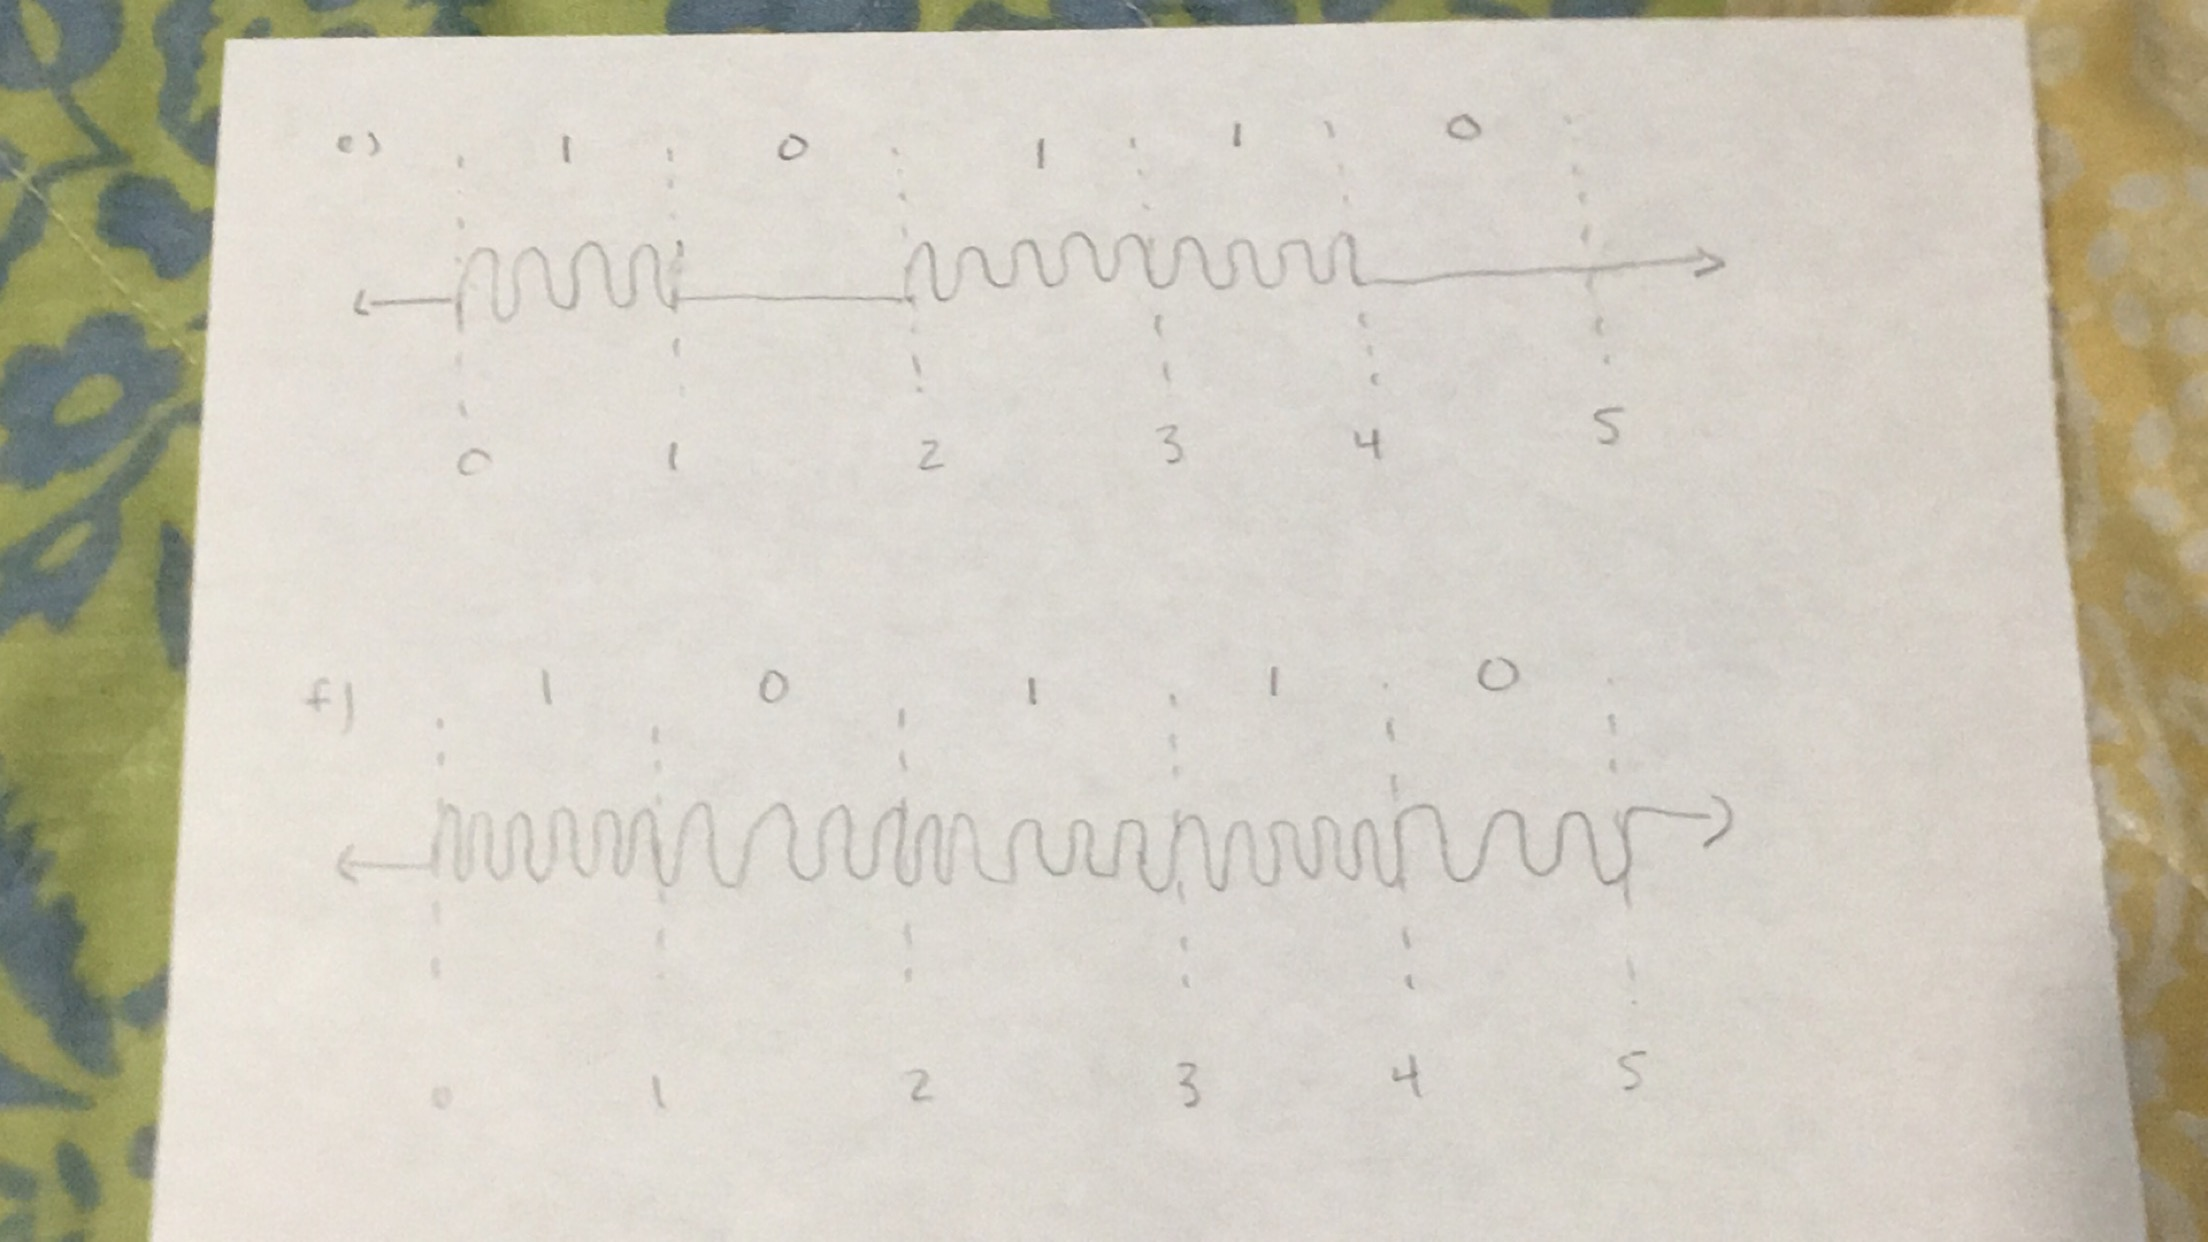
\includegraphics[width=0.5\textwidth]{1ef}
\caption{part (e) and (f)}
\end{figure}

\item {
	For ASK and FSK a signal to noise ratio of $13.5dB$ is needed for a bandwidth efficiency of 1.0
}
\end{enumerate}
 


\section{Channel Capacity, Models}
\begin{enumerate}[label=(\alph*)]

\item {
	$PL(d_0)$ is the frequency dependent component and $\alpha$ is the path loss gradient. The value of $\alpha$ 
	determines how quickly the received signal strength (RSS) falls with distance so the formula 
	$PL(d) = PL(d_0) + 10 * \alpha * log_{10} d/d_0$ makes sense.
}

\item {
	\begin{itemize} \item For $d = 2d_0$: \end{itemize}
	$PL(d) = 40 + 10 * 2.4 * log_{10} (2d_0/d_0) = 40 + 10 * 2.4 * 0.0301 = 47.2247$
	
	\begin{itemize} \item For $d = 4d_0$: \end{itemize}
	$PL(d) = 40 + 10 * 2.4 * log_{10} (4d_0/d_0) = 40 + 10 * 2.4 * 0.0602 = 54.4494$
	
	\begin{itemize} \item Path loss  = 64dB:  \end{itemize}
	Since $40 + 10 * 2.4 = 63$ and $log_{10}10 = 1$ \textbf{then} $d = 10d_0$
}

\item {
	\begin{itemize} \item A $\rightarrow$ B: \end{itemize}
	$10 * log_{10} 10^{-3} - P_{Rx}(dB) = 20dB + (10 * 3) log_{10} 30 - 30 - P_{Rx}(dB) = 64.3 dB$\\
	\textbf{Answer:} $P_{Rx}(dB)$ a + b = $-94.3 dB$
	
	\begin{itemize} \item B $\rightarrow$ C: \end{itemize}
	$-94.3dB - P/a+c = 20dB + 30 * log 20 = 59.03$\\
	\textbf{Answer:} $P$ a+c(dB) = $-153.33 dB$
}

\item {
	Using the equation: $C = B log_2 (1 + SNR)$\\
	$20 * 10^6 = 3 * 10^6 * log_2 (1+SNR)$\\
	$log_2 (1+SNR) = 6.67$\\
	$1 + SNR = 2^{6.67}$\\
	$1+ SNR = 102$\\
	\textbf{Answer: } $SNR = 101$
}

\end{enumerate}


\section{Spread Spectrum and OFDM}
\begin{enumerate}[label=(\alph*)]
\item {
	A spread spectrum system is robust against interference making it beneficial in providing security. It also serves as the basis
	for CDMA technology. Spreading is achieved through frequency hopping. Guard spaces are replaced by the orthogonality of the 
	hopping patterns. Multi-path propagation can be benefited by DSSS systems through recombination which results in a stronger signal. 
}

\item {
	It has orthogonality. Which means the frequency spacing is $\frac{1}{T}$, and if the bit time is T then the base frequency should be
	a multiple of $\frac{1}{T}$
}

\item {
	Main strengths of OFDM include, efficient use of the spectrum through overlap, resistance to frequency selective fading, 
	and the elimination of ISI and IFI through the use of a cyclic prefix. 

}

\item {
	In OFDM the users are allocated only on the time domain. On the other hand OFDMA allows users to be allocated both time 
	and frequency. Thus in OFDMA users will get the best frequencies with the least amount of noise.
}

\item {
	\begin{itemize} 
	\item {
		Adjacent subcarriers: requires measurements to find the best channels but ICI (intercarrier interference) is reduced 
	}
	
	\item {
		Regularly spaced subcarriers: Provides diversification of SNR
	}
	
	\item {
		Randomly spaced subcarriers: Offers all the benefits of regularly spaced subcarriers as well as reduced adjacent cell interference
	}
	\end{itemize}
} 

\item {
	\begin{enumerate} [label=(\arabic*)]
	
	\item {Resiliency against narrow band interface}
	\item {Relatively high security}
	\item {Receiver can separate each user based on code}
	
	\end{enumerate}
}

\item {
	Spread spectrum encodes the signal and then the bandwidth of the signal is increased to reduce jamming of the signal. Thus, 
	the bandwidth is wider after the signal has ben encoded.
}

\item {
	The bandwidth of the signal increases proportionally with the bit rate
}

\item {
	CDMA is "Code Division Multiple Access" and is a spread spectrum technique that allows for signals with a higher bandwidth
	as well as multiple users to be multiplexed over the same channel.
}

\item {
	 Subcarrier spacing: $\frac{1}{T} = \frac{1}{16.67\mu S} = 14.999kHz$ \\
	 Number of required subcarriers: $\frac{bitrate}{subcarrier spacing} = \frac{20 \times 10^6}{10 \times 10^3} = 1333.333$, \\
	 approximating to \textbf{1334 subcarriers}
}

\item {
	$C = B \log_2{1 + SNR}$ \\
	
	\begin{itemize} 
	\item {
		For $SNR = 0.1$ \\
		$B = 0.4MHz$
	}
	
	\item {
		For $SNR = 0.01$ \\
		$B = 3.9MHz$
	}
	
	\item {
		For $SNR = 0.001$ \\
		$B = 38.84MHz$
	}
	\end{itemize}
}
\end{enumerate}
	

\section{Coding and Error Control}
\begin{enumerate}[label=(\alph*)]
\item {0110111 = 0110}

\item {1010101 = 1010}

\item {1110011 = 1110}

\item {1110110 = 1110}

\item {1111100 = 1111} 
\end{enumerate}

\section{Wireshark}
\begin{enumerate}[label=(\alph*)]
\item {
	\begin{enumerate} [label=(\arabic*)]
	
	\item {
		\begin{figure}[h] %[h] means "here" You can put [t] for "top"
		\centering
		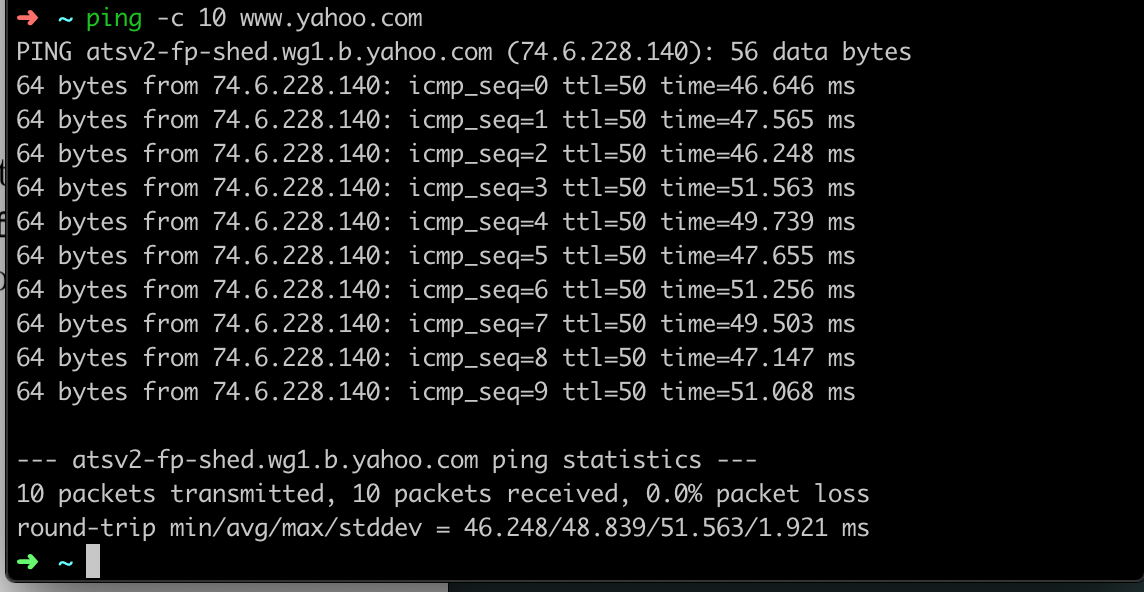
\includegraphics[width=0.5\textwidth]{cmd-output}
		\caption{ping yahoo.com}
		\end{figure}
		Host IP: 192.168.86.38 \\ 
		Destination IP: 74.6.228.140
	}
	
	\item {
		ICMP packets have a type and a code because it communicates network layer information, not application
		layer. The type and code identify the message being received. The network software interprets the messages 
		so no port numbers are needed to direct the messages to a process.
	}
	
	\item {
		\begin{figure}[h] %[h] means "here" You can put [t] for "top"
		\centering
		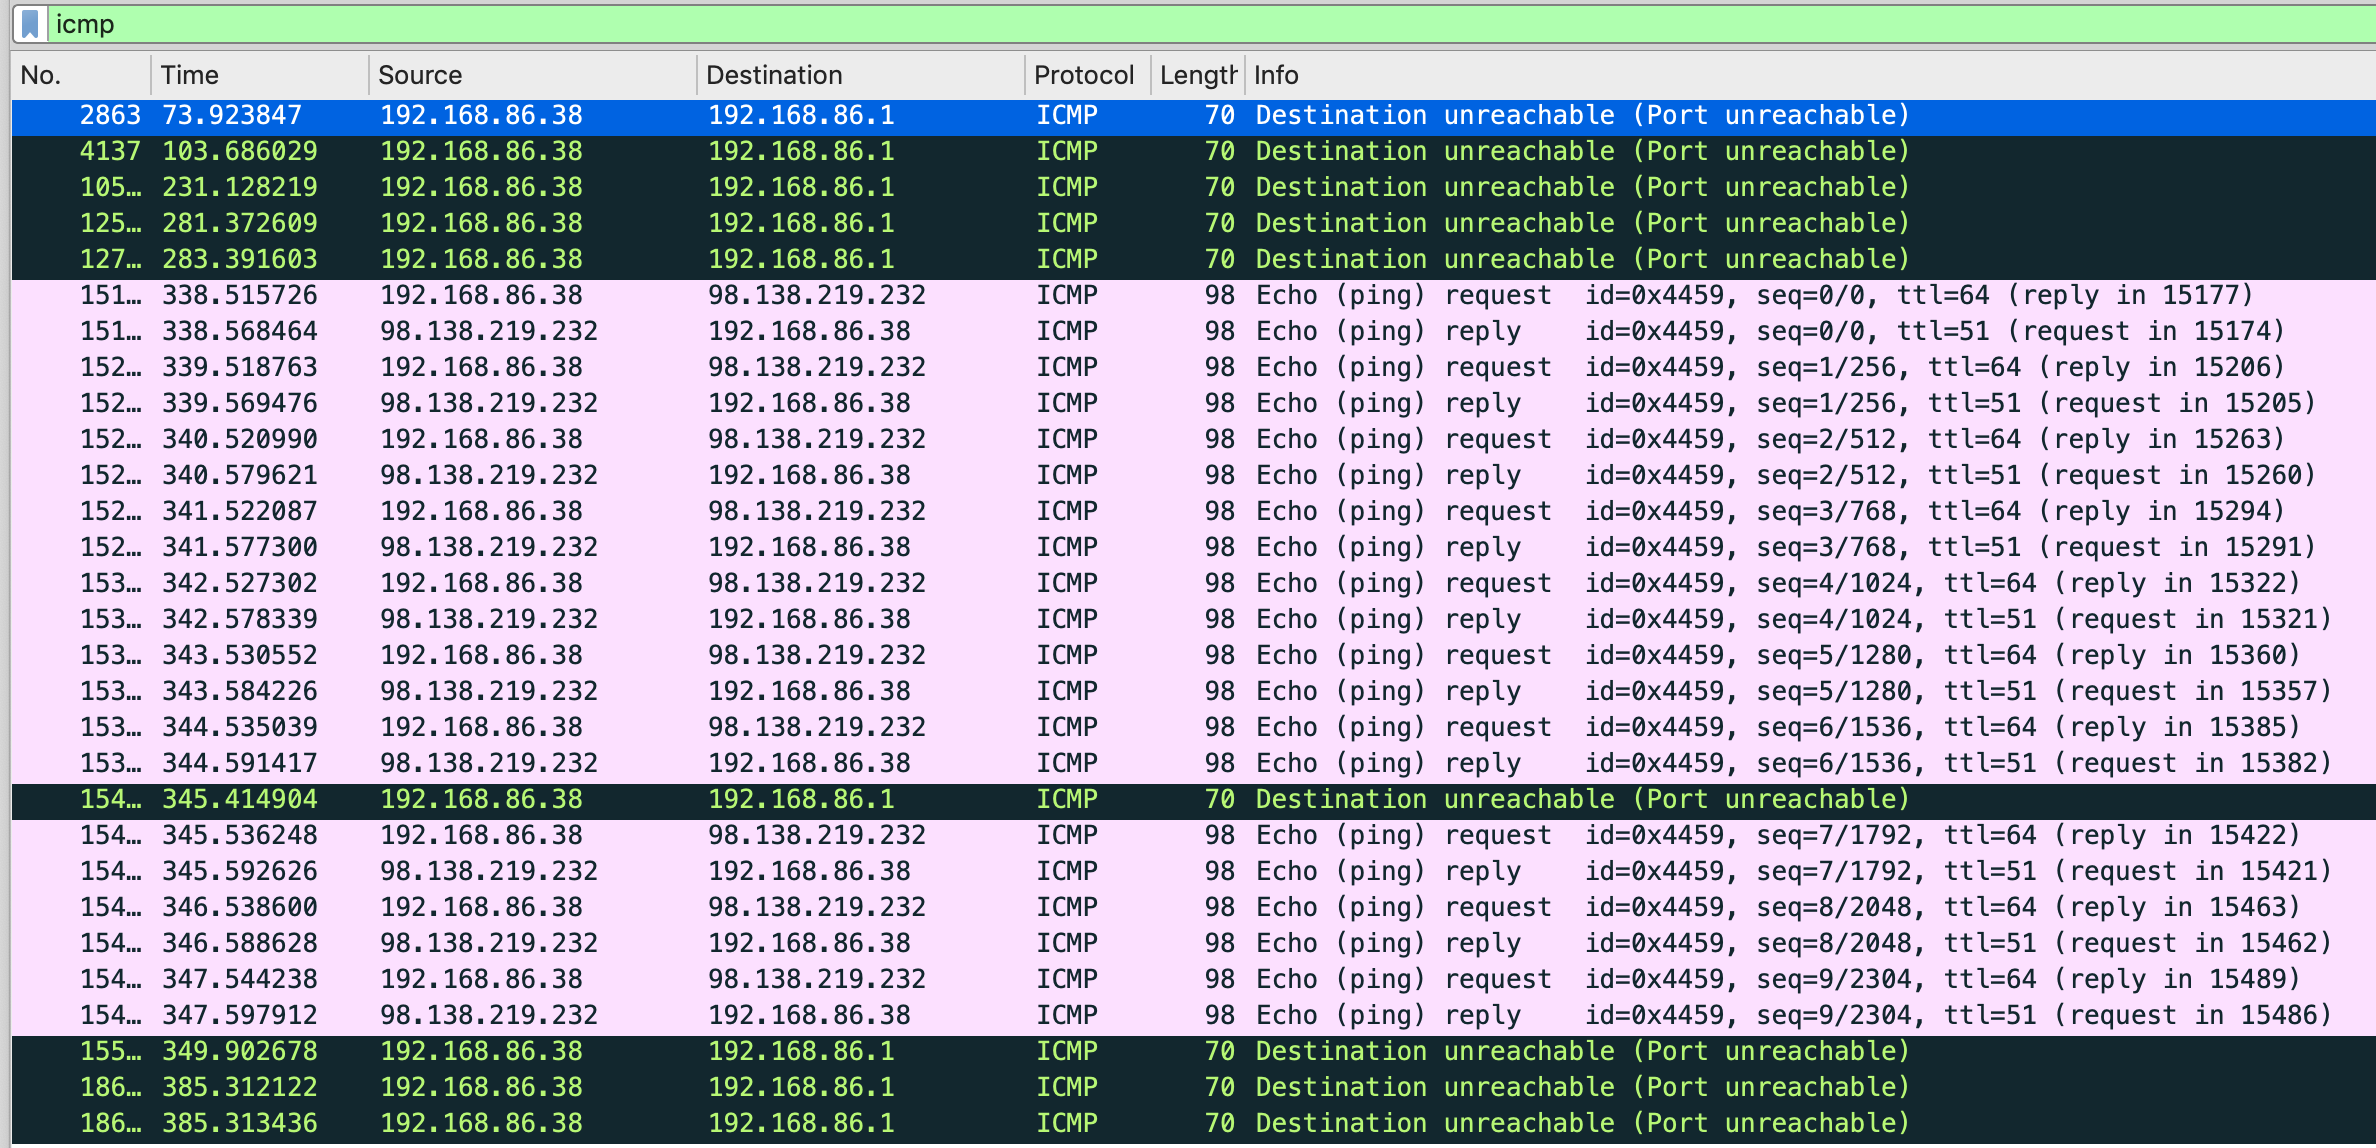
\includegraphics[width=0.5\textwidth]{wireshark-output}
		\caption{icmp output}
		\end{figure}
		
		ICMP Type: 8 Echo (ping) request \\
		Code: 0 \\
		Checksum: 16-bit \\
		Sequence number: 16-bit \\
		Identifier: 16-bit \\
		
		Other fields are the timestamp from the icmp data plus the data itself.
	}
	
	\item {
		ICMP Type: 0 Echo (ping) reply \\
		Code: 0 \\
		Checksum: 16-bit \\
		Sequence number: 16-bit \\
		Identifier: 16-bit \\
		
		Other fields are the timestamp from the icmp data plus the data itself.
	}
	\end{enumerate}
}


\item {
	\begin{enumerate} [label=(\arabic*)]
	\setcounter{enumii}{4}
	
	\item {
		\begin{figure}[h] %[h] means "here" You can put [t] for "top"
		\centering
		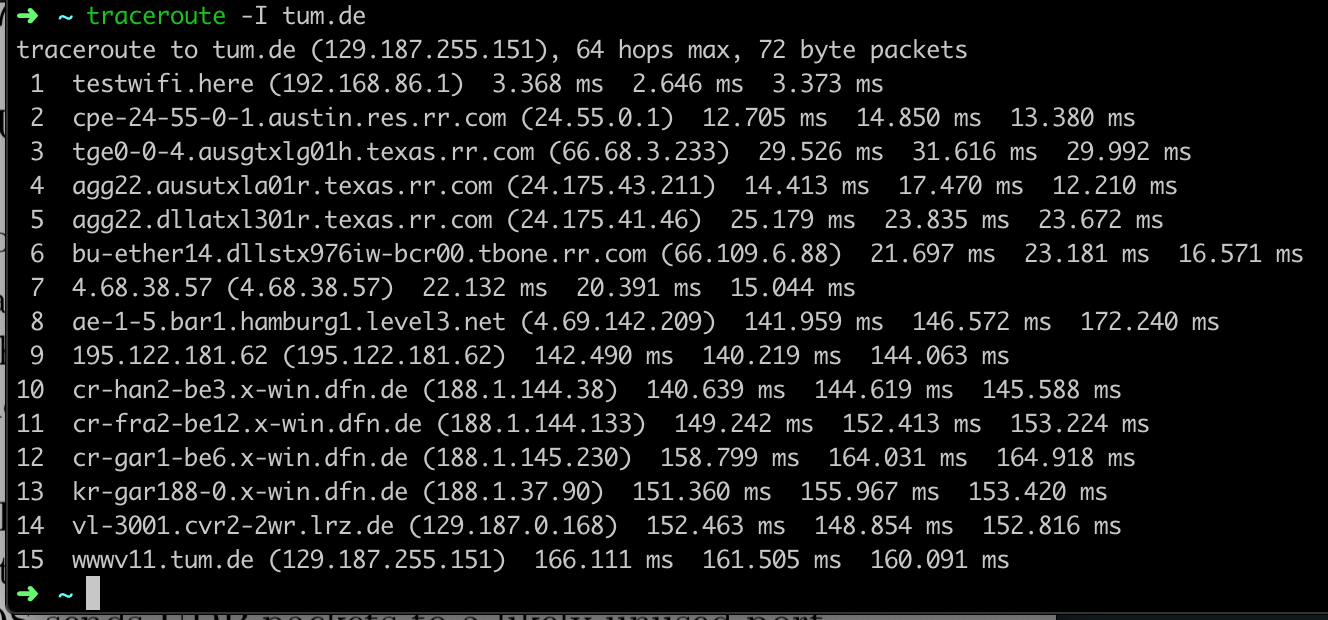
\includegraphics[width=0.5\textwidth]{traceroute-output}
		\caption{traceroute output}
		\end{figure}
		Host IP: 192.168.86.38 \\ 
		Destination IP: 129.187.255.151
	}
	
	\item {
		The protocol number would be 0x11 for UDP instead of 01
	}
	
	\item {
		\begin{figure}[h] %[h] means "here" You can put [t] for "top"
		\centering
		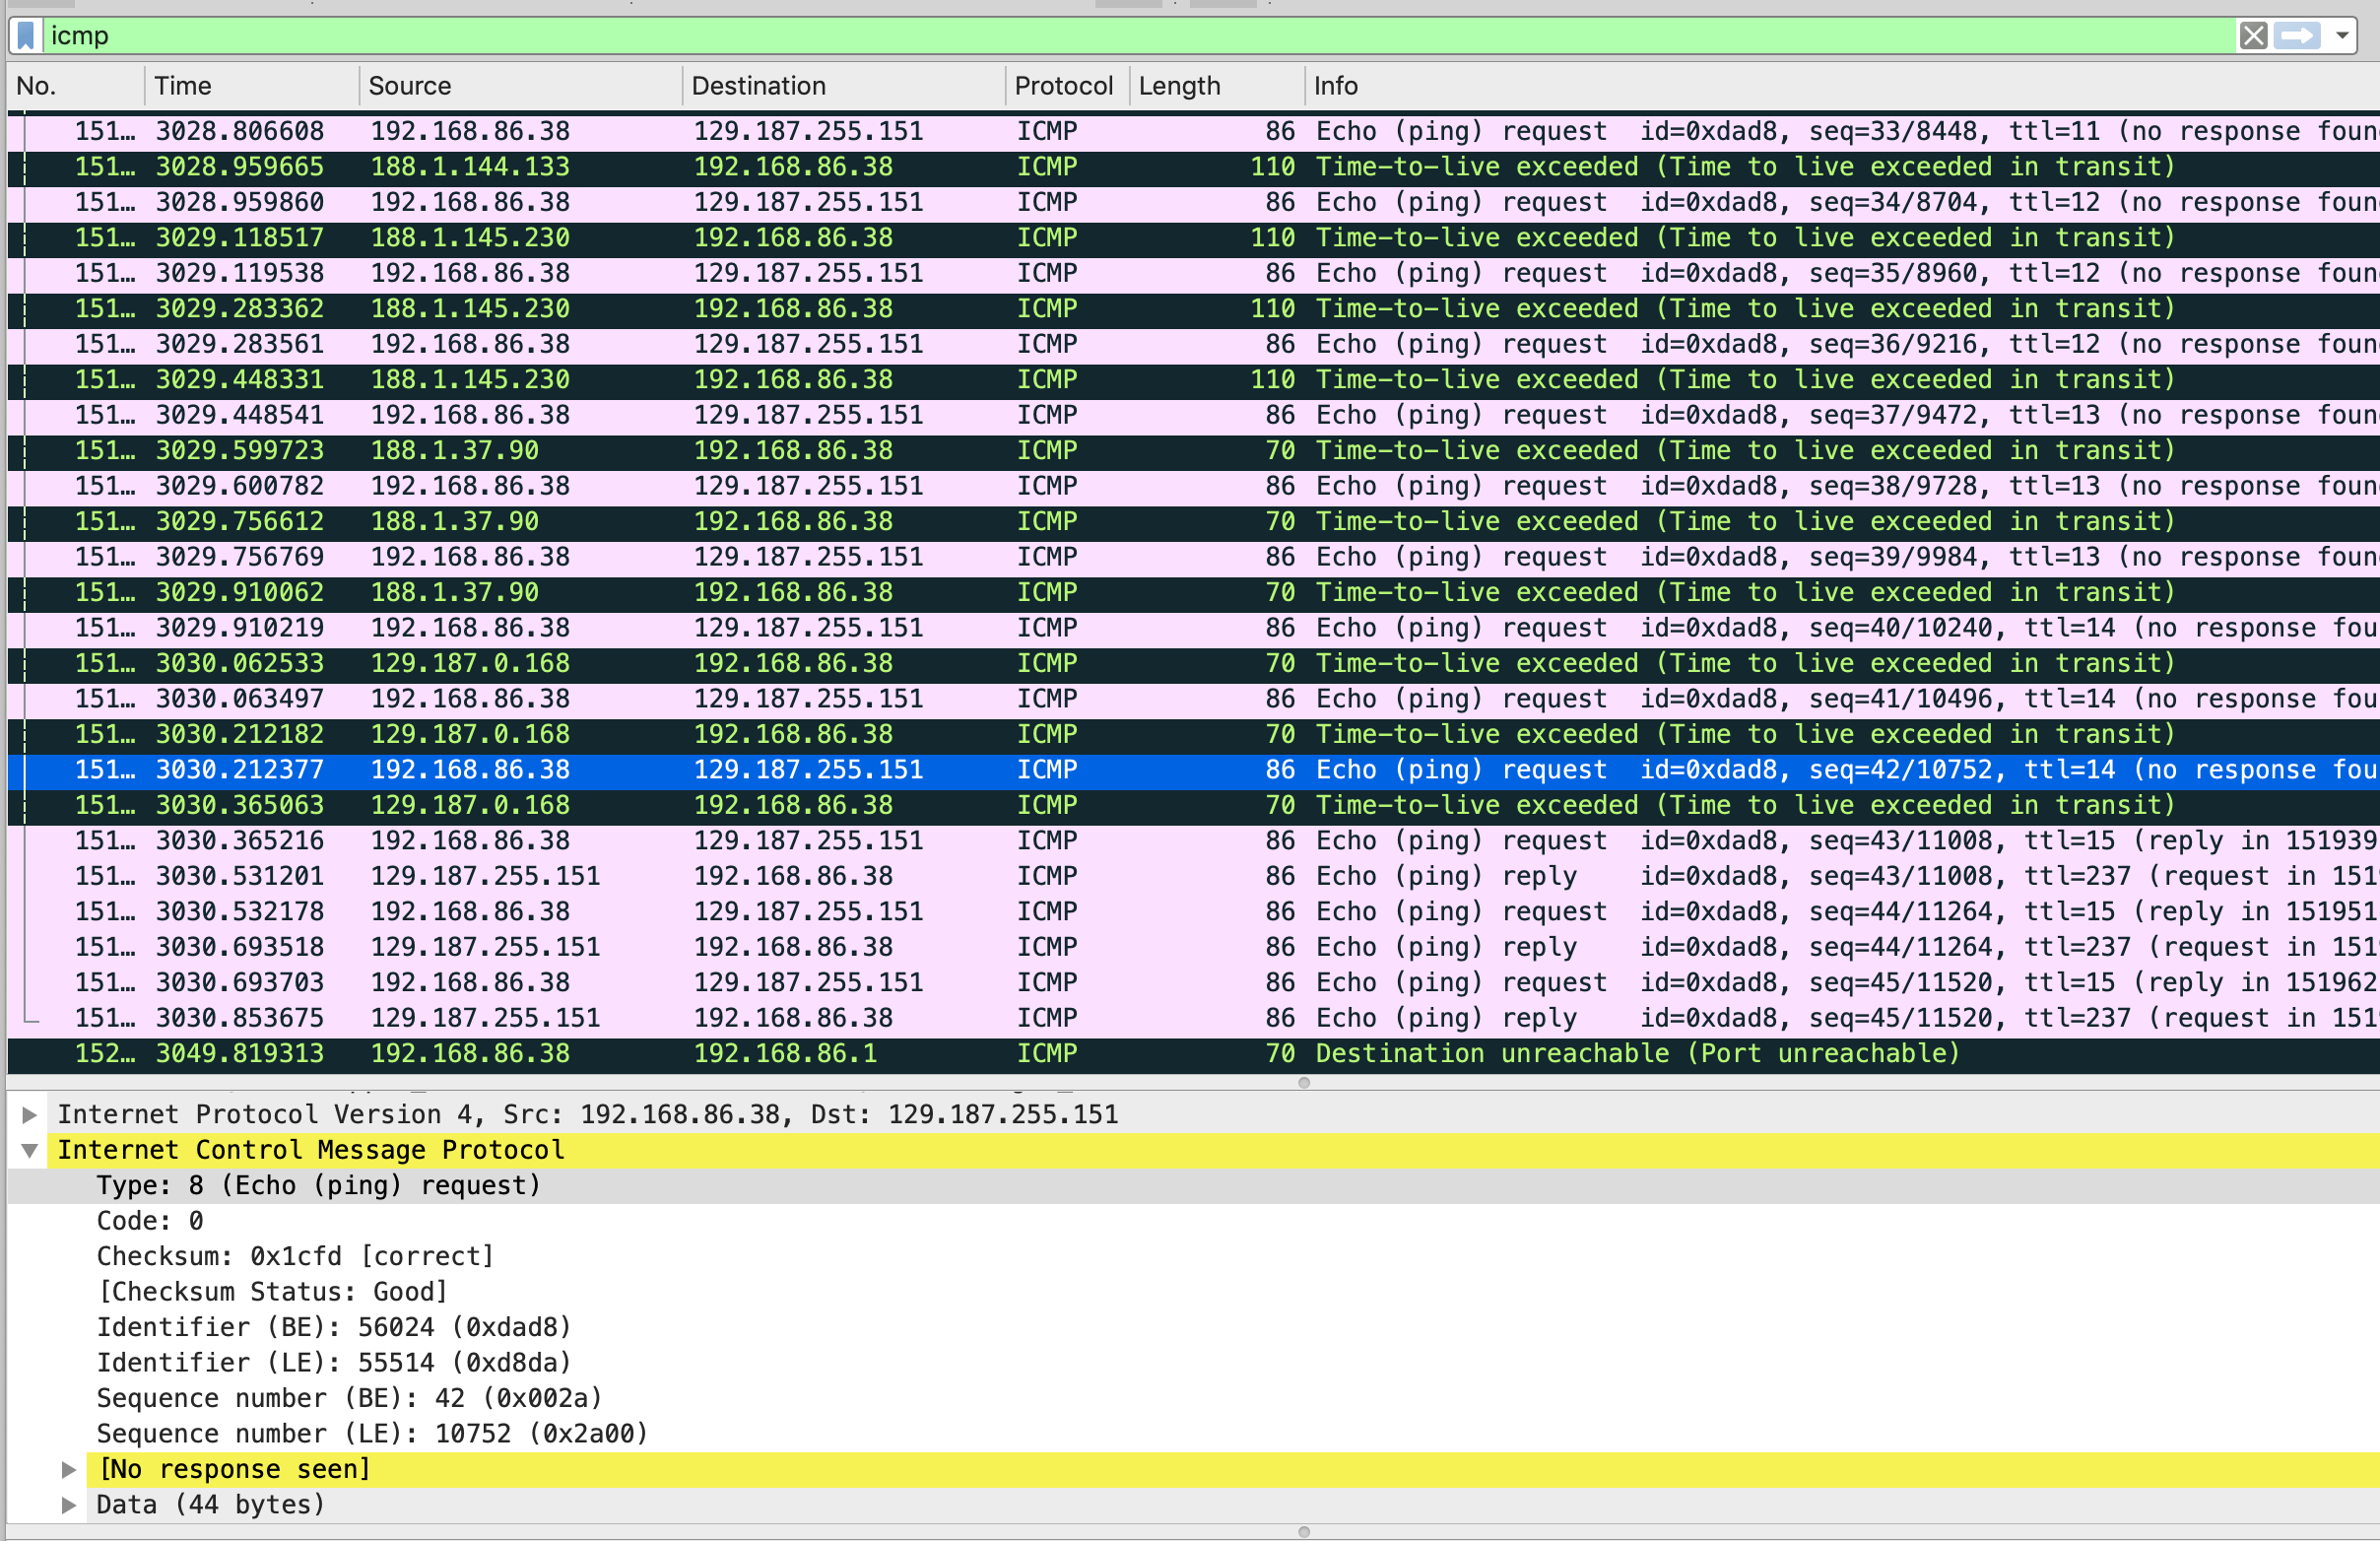
\includegraphics[width=0.5\textwidth]{wireshark-output-2}
		\caption{traceroute wireshark output}
		\end{figure}
		
		The ICMP traceroute echo packet has the same fields as the ping packets
	}
	
	\item {
		\begin{figure}[h] %[h] means "here" You can put [t] for "top"
		\centering
		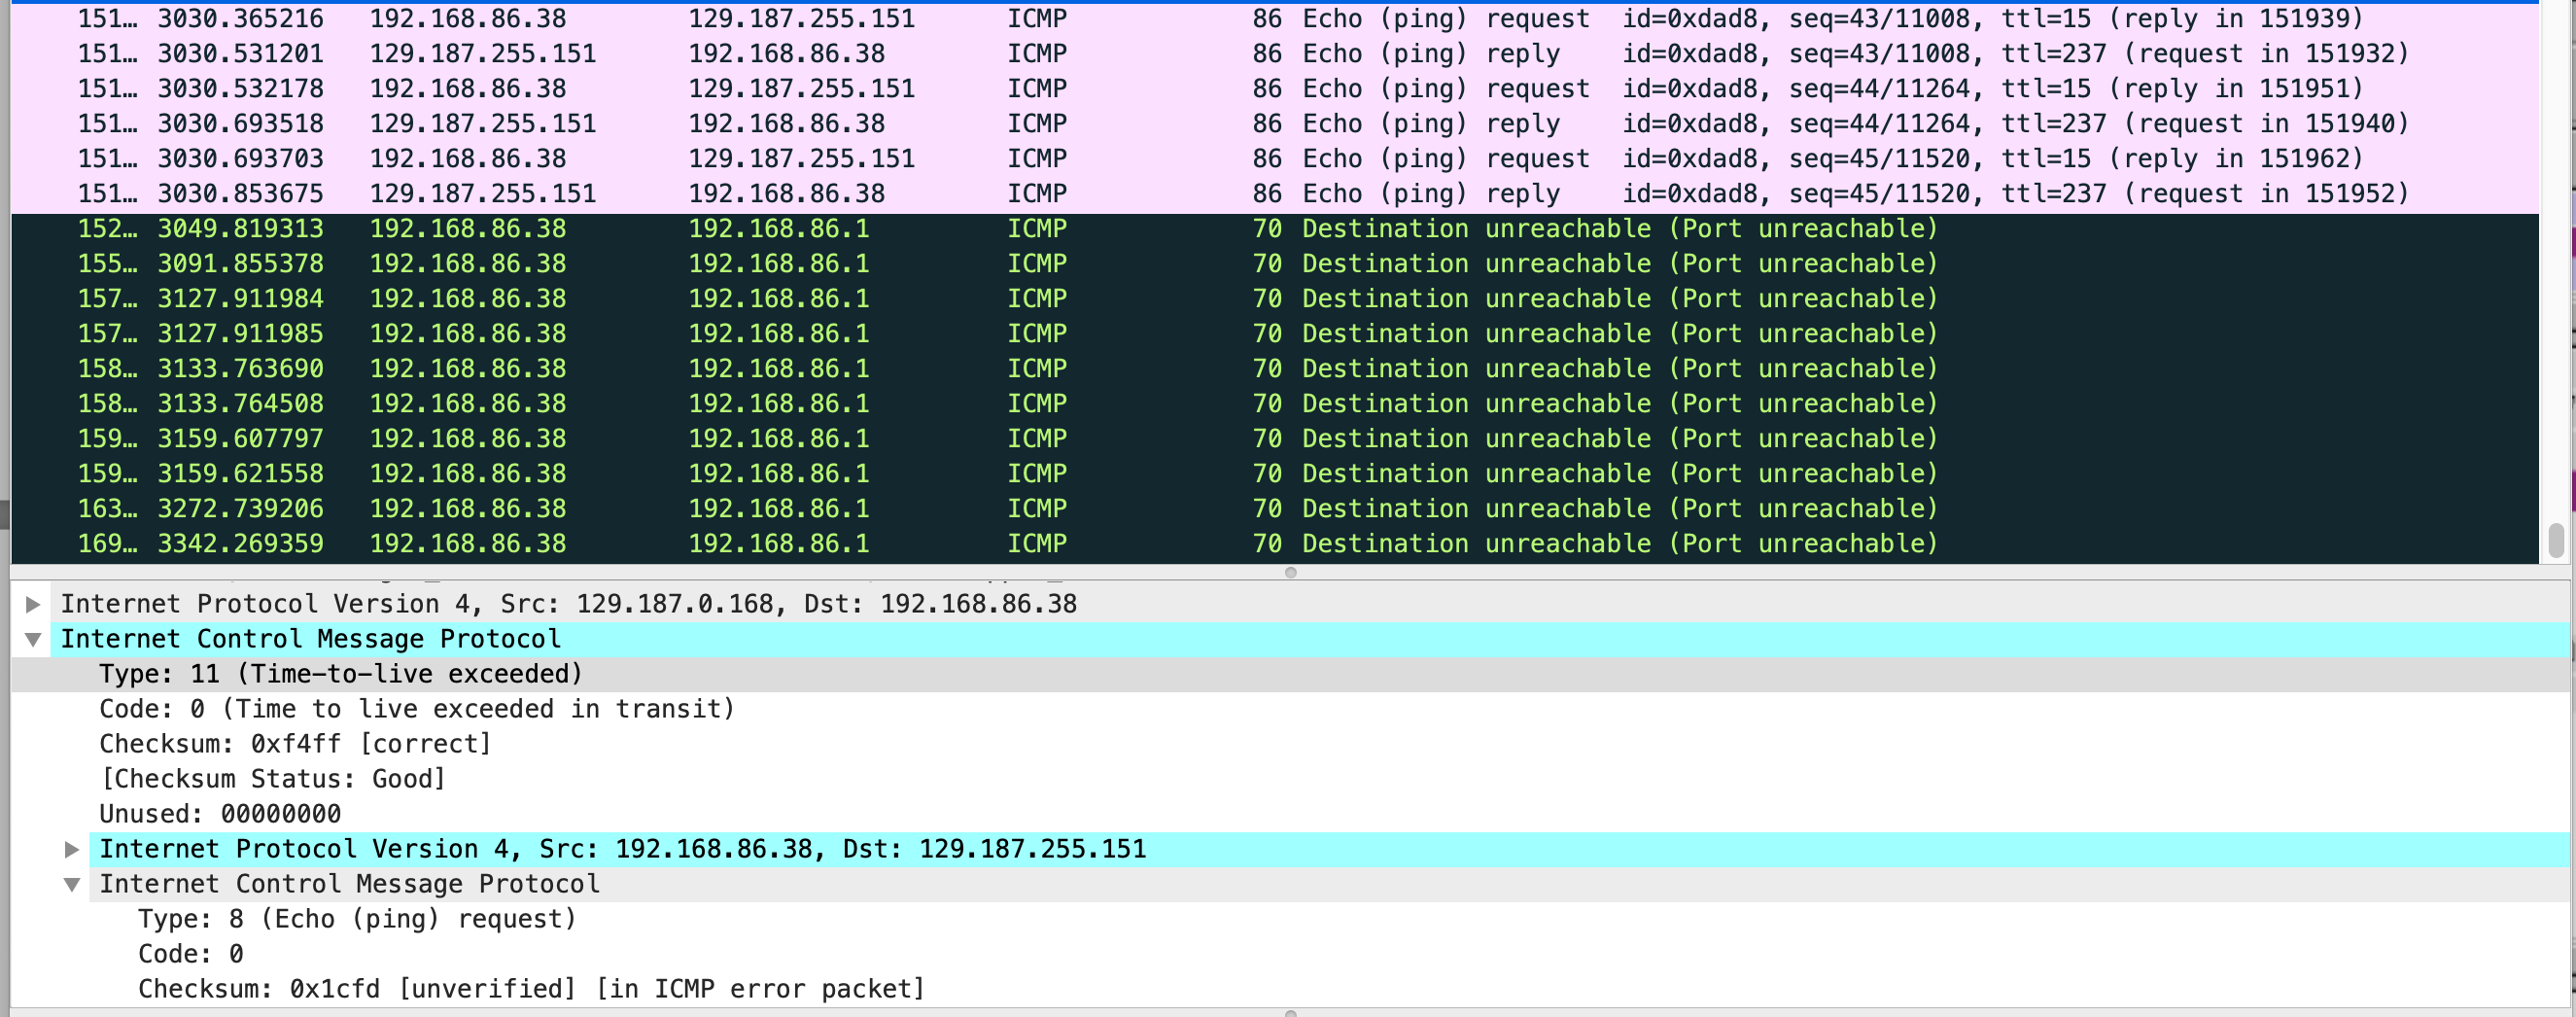
\includegraphics[width=0.5\textwidth]{traceroute-error-output}
		\caption{traceroute error wireshark output}
		\end{figure}
		
		The error packet has a different type than the query packets. It also contains 
		the IP header and the first 8 bytes of the ICMP packet that it is describing.
	}
	
	\item {
		The last three ICMP packets are of type 0 (echo (ping) reply). They are different 
		because the datagrams made it all the way to the destination host before the TTL 
		expired.
	}
	
	\item {
		The longest delay link is between steps 7 and 8. This is a link between US and Hamberg. 
	}
	\end{enumerate}
}
\end{enumerate}

\end{document}

